\section{微分}\label{zhang_differential}
%\begin{figure}[htp]
%    \centering
 %   \begin{tikzpicture}[>=latex]
      %\draw[-](0,0)--(3,0)--(3,3)--(0,3)--(0,0);
      %\draw[-](2,0)--(2,3);
    %  \draw[-](0,2)--(3,2);
   %   \node at(1,1){$A=x_0^2$};
  %\end{tikzpicture}
 % \end{figure}
  \subsection{定义}
  \begin{center}
    设函数$f(x)$在点$x_0$的一个邻域内有定义。$\vartriangle y=f(x_0+\vartriangle x)-f(x_0)$\\\
    如果$\vartriangle y$可以表示为$\vartriangle y=A\vartriangle x+\circ (\vartriangle x)$其中$A$为与$\vartriangle x$无关的常数\\
    则称$f(x)$在点$x_0$可微,$A\vartriangle x$称为$f(x)$在点$x_0$处的微分。\\
    $\mbox{记作:}dy=A\vartriangle x$
  \end{center}
\begin{figure}[htp]
   \centering
    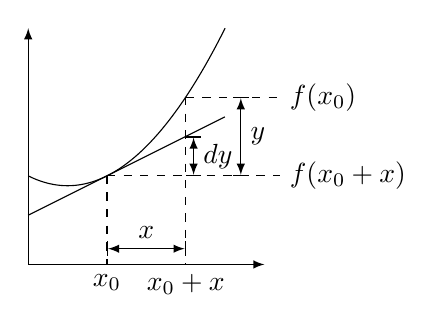
\begin{tikzpicture}[>=latex]
      \draw[->](0,0)--(3,0);
      \draw[->](0,0)--(0,3);
      \draw[domain=0:2.5,samples=1000] plot(\x,{((\x-.5)^2)*(1/2)+1});
      \draw[domain=0:2.5,samples=500] plot(\x,{(\x-1)*(1/2)+9/8});
      \draw[|<->|] (2.1,{(2-1)*(1/2)+9/8})--(2.1,{(((1-.5)^2)*(1/2)+1+(2-1)*(1/2)+9/8)/2})node[right]{$dy$}--(2.1,{((1-.5)^2)*(1/2)+1});
      \draw[dashed](1,{((1-.5)^2)*(1/2)+1})--(1,0)node[below]{$x_0$};
      \draw[dashed](2,{((2-.5)^2)*(1/2)+1})--(2,0)node[below]{$x_0+\vartriangle x$};
     % \node at (3,-1)[below]{常函数\ $f(x)=a\{a\in R\}$};
      \draw[|<->|] (1,.2)--(1.5,.2)node[above]{$\vartriangle x$}--(2,.2);
      \draw[dashed](2,{((2-.5)^2)*(1/2)+1})--(3.2,{((2-.5)^2)*(1/2)+1})node[right]{$f(x_0)$};
      \draw[dashed](1,{((1-.5)^2)*(1/2)+1})--(3.2,{((1-.5)^2)*(1/2)+1})node[right]{$f(x_0+\vartriangle x)$};
      \draw[|<->|](2.7,{((2-.5)^2)*(1/2)+1})--(2.7,{(((2-.5)^2)*(1/2)+1+((1-.5)^2)*(1/2)+1)/2})node[right]{$\vartriangle y$}--(2.7,{((1-.5)^2)*(1/2)+1});
    \end{tikzpicture}
\end{figure}
\begin{align}
    \mbox{可微}\Rightarrow\mbox{可导}\label{differential_to_derivative}\\
    \mbox{可导}\Rightarrow\mbox{可微}\label{derivative_to_differential}
\end{align}

\subsection{微分法则}
\subsubsection{核心根本}
\begin{figure}[htp]
    \centering
    \begin{tikzpicture}[>=latex]
      \draw[->](1.5,.2)--(1.5,.5)--(3,.5)--(3,.2);
      \node at(2.25,.5)[above]{积分};
      \draw[<-](1.5,-.2)--(1.5,-.5)--(3,-.5)--(3,-.2);
      \node at(2.25,-.5)[below]{求导};
      \node at(.5,0){$dy=$};
      \node at(1.5,0){$f'(x)$};
      \node at(2.3,0){$d$};
      \node at(3,0){$x$};
  \end{tikzpicture}
\end{figure}
\subsubsection{四则运算}
\begin{align}
    d\left(u\pm v\right)=du\pm dv\label{differential_operation_rule_1}\\
    d(uv)=vdu+udv \label{differential_operation_rule_2}\\
    d\left(\frac{u}{v}\right)=\frac{vdu+udv}{v^2} \label{differential_operation_rule_3}
\end{align}
\subsubsection{复合运算}
\begin{center}
    可微$\begin{cases}
        y=f(u)\\
        u=g(x)
    \end{cases}\Rightarrow \begin{cases}
        dy=f'(u)du\\
        du=g'(x)dx
    \end{cases}$则$y=f(g(x))$也可微\\
    且$  dy=f'(u)du=f'(u)g(x)dx$\\
    $u$是否为中间变量都成立,微分的不变性。
\end{center}
\subsubsection{近似计算公式}
\begin{center}
    $\vartriangle x\rightarrow 0, dy\approx \vartriangle y\begin{cases}
        dy=f'(x_0)\vartriangle x\\
        \vartriangle y=f(x_0+\vartriangle x)-f(x_0)
    \end{cases}\begin{cases}
        f(x_0+\vartriangle x)\approx f(x_0)+f'(x_0)\vartriangle x\\
        f(x)\approx f(x_0)+f'(x_0)(x-x_0)\\
        x_0=0\begin{cases}
            f(x)\approx f(0)+f'(0)x\\
            \sqrt{n}\approx 1+\frac{1}{n}x\\
            \sin x \approx x\\
            \tan x \approx x\\
            e^x \approx 1+x\\
            \ln(1+n)\approx x
        \end{cases}
    \end{cases}$\\
\end{center}
\subsubsection{奇偶函数导数}
\begin{center}
    偶函数导数为奇函数$f(x)=f(-x)\Leftrightarrow f'(x)=-f'(-x)$\\
    奇函数导数为偶函数$f(x)=-f(-x)\Leftrightarrow f'(x)=f'(-x)$
\end{center}
\subsubsection{区间恒为0}
$$\mbox{若}f'(x)\mbox{在区间恒为零,则}f(x)\mbox{在区间}I\mbox{上为一常数}$$
$\mbox{设}x_1,x_2\mbox{为区间}I\mbox{内任意两点}x_1<x_2$\\
$f(x_2)-f(x_1)=f'(\xi)(x_2-x_1)\equiv 0 $\\
$f(x_2)\equiv f(x_1)=C$
\subsection{中值定理}
\subsubsection{费马引理}
\begin{center}
    $f(x)\qquad \forall x\in \mathring{U}(x_0)\begin{cases}
        f(x)\leqslant f(x_0)\qquad f(x)\mbox{在}x_0\mbox{处取极大值}\\
        f(x)\geqslant f(x_0)\qquad f(x)\mbox{在}x_0\mbox{处取极小值}
    \end{cases}$
\end{center}
\begin{equation}
    \mbox{如果可导函数}y=f(x)\mbox{在}x_0\mbox{取极值,则}f'(x_0)=0\label{Fermat_Lemma}
\end{equation}
\subsubsection{罗尔定理}
\begin{center}
    $\mbox{如果函数}f(x)\mbox{满}\begin{cases}
    \mbox{在闭区间$\left[a,b\right]$上连续}\\
    \mbox{在开区间(a,b)可导}\\
    f(a)=f(b)
    \end{cases}$\\
    \begin{align}
        \mbox{则至少有一点}\xi\in(a,b),f'(\xi)=0\label{Rolle's theorem}
    \end{align}
\end{center}
\begin{figure}[htp]
    \centering
    \begin{tikzpicture}[>=latex,scale=.8]
        \draw[->](-.5,0)--(8,0)node[right]{$x$};
        \draw[->](0,-.5)--(0,4)node[above]{$y$};
        \draw[domain=0:2*pi,samples=1000] plot(\x+1,{sin(\x r)+2});      
        \draw[dashed] (1,{2})--(1,0)node[below]{$a$};    
        \draw[dashed] ({1+(2*pi)},{2})--({1+(2*pi)},0)node[below]{$b$};   
        \draw[dashed] (1,{2})node[left]{$A$}--({1+(2*pi)},{2})node[right]{$B$};
        \draw[dashed] ({1+(.5*pi)},{sin(pi/2 r)+2})--({1+(.5*pi)},0)node[below]{$\xi$};
        \draw[dashed] (1.5,{sin(pi/2 r)+2})--({.5+pi},{sin(pi/2 r)+2});
    \end{tikzpicture}
\end{figure}
\subsubsection{拉格朗日定理$\left(\mbox{微分中值定理}\right)$}
\begin{figure}[htp]
    \centering
    \begin{tikzpicture}[>=latex,scale=.8]
        \draw[->](-.5,0)--(8,0)node[right]{$x$};
        \draw[->](0,-.5)--(0,4)node[above]{$y$};
        \draw[domain=0:2*pi,samples=1000] plot(\x+1,{sin(\x r)+(\x/2)+1});
        \draw[dashed](1,1)--(1,0)node[below]{$a$};
        \draw[dashed]({1+(2*pi)},{(2*pi/2)+1})--({1+(2*pi)},0)node[below]{$b$};
        \draw[dashed](1,1)--({1+(2*pi)},{(2*pi/2)+1});
        \draw[dashed]({1+(pi/2)},{sin(pi/2 r)+(pi/4)+1})--({1+(pi/2)},0)node[below]{$\xi$};
        \draw[dashed]({1+(pi/2)-1},{sin(pi/2 r)+(pi/4)+1-.5})--({1+(pi/2)+1},{sin(pi/2 r)+(pi/4)+1+.5});
    \end{tikzpicture}
\end{figure}
\begin{center}
    $\mbox{如果函数}f(x)\mbox{满}\begin{cases}
    \mbox{在闭区间$\left[a,b\right]$上连续}\\
    \mbox{在开区间(a,b)可导}
    \end{cases}$\\
    $\mbox{则至少有一点}\xi\in(a,b)$\\
    \begin{align}
        f'(\xi)=\frac{f(b)-f(a)}{b-a}\Leftrightarrow f(b)-f(a)=f'(x)(b-a)\label{Lagrange's theorem}
    \end{align}
    在区间$\left[x,x+\vartriangle x\right]$用拉格朗日定理。\\
    $f(x+\vartriangle x)-f(x)=f'(\xi)\vartriangle x$\\
    $\xi\in(x,x+\vartriangle x)$记作:\ $\xi=x+\theta \vartriangle x\qquad 0<\theta <1$\\
    $f(x+\vartriangle x)-f(x)=f(x+\theta \vartriangle x)\vartriangle x$\\
    $\vartriangle y=f(x+\theta \vartriangle x)\vartriangle x$\\

\end{center}
\subsubsection{柯西定理}
\vspace{-3mm}
\begin{figure}[htp]
    \centering
    \begin{tikzpicture}[>=latex,scale=.8]
        \draw[->](-.5,0)--(8,0)node[right]{$X$};
        \draw[->](0,-.5)--(0,5)node[above]{$Y$};
        \draw[domain=0:2*pi,samples=1000] plot(\x+1,{sin(\x r)+(\x/2)+1});
        \draw[dashed](1,1)--(1,0)node[below]{$F(a)$};
        \draw[dashed]({1+(2*pi)},{(2*pi/2)+1})--({1+(2*pi)},0)node[below]{$F(b)$};
        \draw[dashed](1,1)--({1+(2*pi)},{(2*pi/2)+1});
        \node at(.8,1.3){A};\node at({1.2+(2*pi)},{(2*pi/2)+1}){B};
        \draw[dashed](1,1)--(0,1)node[left]{$f(a)$};
        \draw[dashed]({1+(2*pi)},{(2*pi/2)+1})--(0,{(2*pi/2)+1})node[left]{$f(b)$};
        \draw[dashed]({1+(pi/2)},{sin(pi/2 r)+(pi/4)+1})--({1+(pi/2)},0)node[below]{$F(\xi)$};
        \draw[dashed]({1+(pi/2)-1},{sin(pi/2 r)+(pi/4)+1-.5})--({1+(pi/2)+1},{sin(pi/2 r)+(pi/4)+1+.5});
    \end{tikzpicture}
\end{figure}
\begin{center}
    $\mbox{如果函数}f(x)\mbox{满}\begin{cases}
    \mbox{在闭区间$\left[a,b\right]$上连续}\\
    \mbox{在开区间(a,b)可导}\\
    F'(x)\neq 0
    \end{cases}\quad\mbox{参数方程}(a\leqslant x \leqslant b)\begin{cases}
        X=F(x)\\
        Y=f(x)
    \end{cases}$
\end{center}
\begin{equation}
    \mbox{至少有一点,} \xi\qquad\frac{f'(\xi)}{F'(\xi)}=\frac{f(b)-f(a)}{F(b)-F(a)}\label{cauchy_theorem}
\end{equation}
\begin{displaymath}
    \begin{split}
    \mbox{切线斜率}&=\frac{dY}{dX}=\frac{df(x)}{dF(x)}=\frac{f'(x)}{F'(x)}\Rightarrow x=\xi\mbox{时斜率}=\frac{f'(\xi)}{F'(\xi)}\\
    AB\mbox{的斜率}&=\frac{f(b)-f(a)}{F(b)-F(a)}
    \end{split}
\end{displaymath}
\subsubsection{三个定理关系}
$$\frac{f'(\xi)}{F'(\xi)}=\frac{f(b)-f(a)}{F(b)-F(a)},(F(x)=x)\Rightarrow f'(\xi)=\frac{f(b)-f(a)}{b-a},(f(b)=f(a))\Rightarrow f'(\xi)=0$$
\subsection{洛必达法则}
$$\mbox{未定型},\quad\frac{0}{0},\quad\frac{\infty}{\infty},\quad0^0,\quad1^\infty,\quad\infty^0,\quad\infty-\infty$$
\begin{center}
    $\lim\limits_{x\to x_0}\frac{f(x)}{F(x)}=\lim\limits_{x\to x_0}\frac{f'(x)}{F'(x)}\begin{cases}
    \lim\limits_{x\to x_0}f(x)=0,\lim\limits_{x\to x_0}F(x)=0\\
    f(x),F(x)\mbox{在}x_0\mbox{的某去心邻域内可导,且}F'(x)\neq 0\\
    \lim\limits_{x\to x_0}\frac{f'(x)}{F'(x)}\mbox{存在,或无穷小。则}
\end{cases}$
\end{center}
\begin{equation}
    \lim\limits_{x\to x_0}\frac{f(x)}{F(x)}=\lim\limits_{x\to x_0}\frac{f'(x)}{F'(x)}\label{l'hospital rule}
\end{equation}
    \begin{center}
        $\lim\limits_{x\to \infty}\frac{f(x)}{F(x)}=\lim\limits_{x\to \infty}\frac{f'(x)}{F'(x)}\begin{cases}
        \lim\limits_{x\to x_0}f(x)=0,\lim\limits_{x\to x_0}F(x)=0\\
        \exists N\ \mbox{当}\left|x\right|>N\mbox{,时}f'(x),F'(x)\mbox{存在,且}F'(x)\neq 0\\
        \lim\limits_{x\to x_0}\frac{f'(x)}{F'(x)}\mbox{存在,或为无穷大。则}
    \end{cases}$
\end{center}
\subsection{泰勒公式}
\begin{displaymath}
    \begin{split}
        f(x_0+\vartriangle x)-f(x_0)&=f'(x_0)\vartriangle x +\circ (\vartriangle x)\\
        x_0+\vartriangle &= x \qquad \vartriangle x= x-x_0\\
        f(x)-f(x_0)&=f'(x_0)(x-x_0) +\circ (\vartriangle x)\\
        f(x)&=f'(x_0)(x-x_0)+f(x_0)+\circ (\vartriangle x)\\
        f(x)&\approx f'(x_0)(x-x_0)+f(x_0)
    \end{split}\quad
    \begin{split}
        P(x_0)&=f(x_0) \\
        P'(x_0)&=f'(x_0)\\
    \end{split}
\end{displaymath}
\subsubsection{泰勒多项式}
\centerline{$P(x)=a_0+a_1(x-x_0)+a_2(x-x_0)^2+\cdots+a_n(x-x_0)^n\mbox{去近似某个多项式}$}
$\begin{cases}
    P_n(x_0)&=f(x_0)=a_0\\
    P_n'(x_0)&=f'(x_0)=a_1\\
    P_n''(x_0)&=f''(x_0)=a_2\cdot 2!\\
    &\vdots \\
    P_n^{(n-1)}(x_0)&=f^{(n-1)}(x_0)=a_{n-1}\cdot(n-1)!\\
    P_n^{(n)}(x_0)&=f^{(n)}(x_0)=a_n\cdot n!\\
\end{cases}\Rightarrow\begin{cases}
    a_0&= f_n(x_0)\\
    a_1&=f_n'(x_0)\\
    a_2&=\frac{f_n''(x_0)}{2!}\\
    &\vdots \\
    a_{n-1}&=\frac{f_n^{(n-1)}(x_0)}{(n-1)!}\\
    a_n&=\frac{f_n^{(n)}(x_0)}{n!}
\end{cases}$
$$P_n(x)=f(x_0)+f'(x_0)(x-x_0)+\frac{f''(x_0)}{2!}(x-x_0)^2\cdots\frac{f^{(n-1)}(x_0)}{(n-1)!}(x-x_0)^{n-1}+\frac{f^n(x_0)}{n!}(x-x_0)^n$$
\centerline{$f(x)\approx P_n(x)$}
\subsubsection{泰勒中值定理}
$\mbox{如果}{f(x)|x_0\in (a,b)}\mbox{内有}(n+1)\mbox{阶导则}$
\begin{displaymath}
    \begin{split}
        f(x)&=P_n(x)+R_n(x) \\
        P_n(x)&=f(x_0)+f'(x_0)(x-x_0)+\frac{f''(x_0)}{2!}(x-x_0)^2+\cdots+\frac{f^n(x_0)}{n!}(x-x_0)^n+R_n(x)\\
    \end{split}
\end{displaymath}
\centerline{拉格朗日余项}
\begin{equation}
    R_n(x)=\frac{f^{(n+1)}(\xi)}{(n+1)!}(x-x_0)^{n+1}\qquad \{\xi\in(x,x_0)\} \label{lagrange_remainder}
\end{equation}
\centerline{皮亚诺于项}
\begin{equation}
    R_n(x)=\circ(\left|x-x_0\right|^n) \label{Piano_remainder}
\end{equation}
\centerline{$f(x)\approx P_n(x)$误差为$R_n(x)$}
\subsection{麦克劳林公式}
\begin{center}
    $x_0=0$\\
    $P_n(x)= f(0)+f'(0)x+\frac{f''(0)}{2!}x^2+\cdots+\frac{f^n(0)}{n!}x^n+\begin{cases}
        \frac{f^{(n+1)}(\theta x)}{(n+1)!}x^{n+1}.\ 0<\theta<1\\
        \circ(\left|x\right|^n)
    \end{cases}$
\end{center}
\subsubsection{常用的麦克劳林展开}
\begin{displaymath}
    \begin{split}
        e^x&=1+1x+\frac{1}{2!}x^2+\cdots+\frac{1}{n!}x^n\begin{cases}
        \frac{f^{(n+1)}(\theta x)}{(n+1)!}x^{n+1}.\ 0<\theta<1\\
        \circ(\left|x\right|^n)\end{cases}\\
    \sin x&=1x-\frac{1}{3!}x^3+\frac{1}{5!}x^5-\frac{1}{7!}x^7+\cdots+(-1)^{n-1}\frac{1}{(2n-1)!}x^{2n-1}+R_n(x)\\
    \cos x&=1-\frac{1}{2!}x^2+\frac{1}{4!}x^4-\frac{1}{6!}x^6\cdots+(-1)^{n}\frac{1}{(2n)!}x^{2n}+R_n(x)\\
    \ln(1+x)&=x-\frac{1}{2}x^2+\frac{1}{3}x^3-\frac{1}{4}x^4\cdots+(-1)^{n-1}\frac{1}{n}x^{n}+R_n(x)\\
        \ln(1-x)&=-x-\frac{1}{2}x^2-\frac{1}{3}x^3-\frac{1}{4}x^4\cdots-\frac{1}{n}x^{n}+R_n(x)\\
    (1+x)^\alpha&=1+\alpha x+\frac{\alpha(\alpha-1)}{2!}x^2+\frac{\alpha(\alpha-1)(\alpha-2)}{3!}x^3\cdots\frac{A_\alpha^n}{n!}x^n+R_n(x)
    \end{split}
\end{displaymath}



